\section{直线的基本概念}

\begin{definition}[斜截式]
    已知斜率 $k$，已知截距 $b$，其标准方程为 $y=kx+b$，其中 $k$ 是存在的。

    \begin{tips}
        注意斜率的取值范围应该是 $(-\infty, +\infty)$
    \end{tips}

\end{definition}

\begin{theorem}[两点间的斜率公式]
    已知两点 $A(x_1, y_1)$ 和 $B(x_2, y_2)$，则直线 $AB$ 的斜率为 $k = \frac{y_2 - y_1}{x_2 - x_1}$，其中 $x_2 \neq x_1$.
\end{theorem}

\begin{example}
    求两点之间形成的斜率：
    \begin{itemize}
        \item 求点 $(3,-4)$ 和点 $(1,2)$ 两点形成的斜率。
        \item 求点 $(m, 2)$ 和点 $(m-2, 1)$ 两点形成的斜率。
    \end{itemize}
\end{example}

\v{2em}

\begin{example}
    若 $A(1,2), B(-1,0), C(m, 3)$ 三点在同一条直线上，则实数 $m=$（\quad）
    \begin{tasks}(4)
        \task $-2$
        \task $-1$
        \task $0$
        \task $1$
    \end{tasks}
\end{example}

\v{2em}

\begin{theorem}[平面上的点的约束关系]
    $(x,y)$ 是被约束的，所以只要给出一个 $f(x,y)$ 就能描述这个点的轨迹。
\end{theorem}

\begin{example}
    请说出 $3y-x+6=0$ 的点的约束关系。
\end{example}

\v{2em}

\begin{definition}[直线的倾斜角]
    直线的倾斜角 $\theta$ 是指直线与 $x$ 轴正方向之间的夹角，满足 $\tan \theta = k$，其中 $k$ 是直线的斜率。

    \begin{center}
        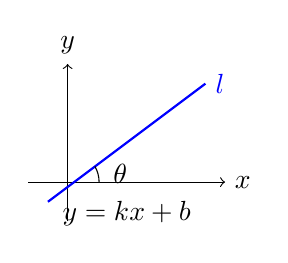
\begin{tikzpicture}[scale=0.5]
            % 绘制坐标轴
            \draw[->] (-1,0) -- (4,0) node[right] {$x$};
            \draw[->] (0,-1) -- (0,3) node[above] {$y$};

            \draw[thick, blue] (-0.5,-0.5) -- (3.5,2.5) node[right] {$l$};
            \draw (0.8,0) arc (0:30:0.8) node[midway, right=2pt] {$\theta$};
            \node at (1.5,-0.8) {$y = kx + b$};
        \end{tikzpicture}
    \end{center}

    \begin{tips}
        直线的倾斜角的取值范围应为 $[0, \pi)$，
    \end{tips}
\end{definition}

\begin{example}
    直线 $l_1: x+5=0$ 与直线 $l_2: 3 x+\sqrt{3} y+2=0$ 的夹角的大小为 \underline{$\qquad$}.
\end{example}

\v{4em}

\begin{example}
    直线 $l$ 的方程为 $x-y \cos \theta+2=0$ ，则直线 $l$ 的倾斜角 $\alpha$ 的取值范围是（ \quad）
    \begin{tasks}(4)
        \task $[0, \pi]$
        \task $\left[\frac{\pi}{4}, \frac{\pi}{2}\right]$
        \task $\left[\frac{\pi}{4}, \frac{3 \pi}{4}\right]$
        \task $\left[\frac{\pi}{4}, \frac{\pi}{2}\right) \cup\left(\frac{\pi}{2}, \frac{3 \pi}{4}\right]$
    \end{tasks}
\end{example}

\v{4em}

\begin{example}
    已知两点 $A(a, 3), B(1,-2)$ ，若直线 $A B$ 的倾斜角为 $135^{\circ}$ ，则 $a$ 的值为（\quad）
    \begin{tasks}(4)
        \task -6
        \task  6
        \task -4
        \task  4
    \end{tasks}
\end{example}

\vspace{2em}

\begin{theorem}[倾斜角与斜率的关系]
    直线的倾斜角 $\alpha$ 的范围是 $[0, \pi)$。斜率 $k = \tan\alpha$。
    \begin{enumerate}
        \item 当 $\alpha \in [0, \pi/2)$ 时，$k \ge 0$ 且 $k$ 随 $\alpha$ 增大而增大；
        \item 当 $\alpha \in (\pi/2, \pi)$ 时，$k < 0$ 且 $k$ 随 $\alpha$ 增大而增大。
    \end{enumerate}
\end{theorem}

\begin{example}
    直线 $l_1, l_2, l_3$ 的斜率分别为 $k_1, k_2, k_3$ ，倾斜角分别为 $\alpha_1, \alpha_2, \alpha_3$ ，则下列选项正确的是（\hspace{2em}）

    \begin{figure} [H]
        \centering
        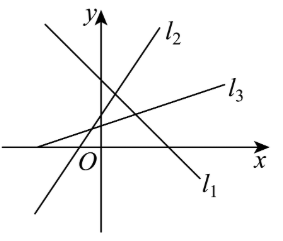
\includegraphics[width=0.15\textwidth]{chapters/直线与圆/images/直线与圆的基本概念/img-20250707161548.png}
    \end{figure}

    \begin{tasks}(4)
        \task $k_1<k_3<k_2$
        \task $k_3<k_2<k_1$
        \task $\alpha_1<\alpha_3<\alpha_2$
        \task $\alpha_3<\alpha_2<\alpha_1$
    \end{tasks}
\end{example}

\begin{theorem}[两条直线之间的夹角公式]
    已知两条直线 $l_1: y = k_1 x + b_1$ 和 $l_2: y = k_2 x + b_2$，则它们之间的夹角 $\theta$ 满足 $\tan \theta = \left| \frac{k_1 - k_2}{1 + k_1 k_2} \right|$，其中 $k_1 k_2 \neq -1$.
\end{theorem}

\begin{example}
    若直线 $l_1, l_2$ 的斜率是方程 $x^2+x-6=0$ 的两根，则这两条直线的夹角为（ \qquad）
    \begin{tasks}(4)
        \task $\frac{\pi}{4}$
        \task $\frac{\pi}{6}$
        \task $\frac{\pi}{3}$
        \task $\frac{\pi}{2}$
    \end{tasks}
\end{example}

\v{8em}

\begin{example}
    已知直线过点 $P(-4,1)$ ，且与直线 $m: 3 x-y+1=0$ 的夹角为 $\arccos \frac{3 \sqrt{10}}{10}$ ，求直线 $l$ 的方程．
\end{example}

\v{8em}

\begin{definition}[一般式]
    已知 $A, B$ 不同时为 $0$，其标准方程为 $Ax+By+C=0$.

    一般式非常通用，可以直接表示任何直线（不需要讨论斜率不存在的情况）。
\end{definition}

\begin{example}
    直线 $x-\sqrt{3} y+1=0$ 的一个方向向量是（\quad ）。
    \begin{tasks}(4)
        \task $(1, \sqrt{3})$
        \task $(\sqrt{3}, 1)$
        \task $(1, -\sqrt{3})$
        \task $(-\sqrt{3}, 1)$
    \end{tasks}
\end{example}

\begin{tips}
    如果再求该直线的一个法向量呢？
\end{tips}

\v{4em}

\begin{definition}[点斜式]
    已知直线的斜率 $k$ 和直线上一点 $(x_0, y_0)$，则直线的方程为 $y - y_0 = k(x - x_0)$。
\end{definition}

\begin{warning}
    这将是高中阶段最重要的式子！请务必熟记。
\end{warning}

\v{2em}

\begin{example}
    已知 $\triangle A B C$ 的三个顶点是 $A(1,4), B(5,7), C(7,-4)$
    \begin{itemize}
        \item （1）求 $B C$ 边上的中线的直线方程；
        \item （2）求 $B C$ 边上的高的直线方程
    \end{itemize}
\end{example}

\v{12em}

\begin{definition}[两点式]
    已知两点 $A(x_1, y_1)$ 和 $B(x_2, y_2)$，则直线 $AB$ 的方程为 $\frac{y-y_1}{y_2-y_1} = \frac{x-x_1}{x_2-x_1}$，其中 $x_2 \neq x_1$ 且 $y_2 \neq y_1$.
\end{definition}

\begin{example}
    用两点式来表达直线的方程：
    \begin{itemize}
        \item 已知点 $A(1,2)$ 和点 $B(3,4)$，求直线 $AB$ 的方程。
        \item 求经过两点 $A(2,m)$ 和 $B(n,3)$ 的直线方程。
    \end{itemize}
\end{example}

\v{6em}

\begin{definition}[截距式]
    已知 $x, y$ 轴上的截距 $a, b$ 且 $ab \neq 0$，其标准方程为 $\frac{x}{a} + \frac{y}{b} = 1$。

    其中直线既不能垂直于 $x$ 轴，也不能垂直于 $y$ 轴，且不过原点。
\end{definition}

\begin{example}
    求过点 $(4,-3)$ 且在两坐标轴上截距相等的直线 $l$ 的方程。
\end{example}

\begin{solution}
    设直线在 $x$ 轴、 $y$ 轴上的截距分别为 $a, b$ ．

    （1）当 $a \neq 0, b \neq 0$ 时，设 $l$ 的方程为 $\frac{x}{a}+\frac{y}{b}=1$. \\
    $\because$ 点 $(4,-3)$ 在直线上，$\therefore \frac{4}{a}-\frac{3}{b}=1$ ，
    若 $a=b$ ，则 $a=b=1$ ，直线方程为 $x+y-1=0$ ．

    （2）当 $a=b=0$ 时，直线过原点，且过点 $(4,-3)$. \\
    $\therefore$ 直线的方程为 $3 x+4 y=0$ ．
    综上知，所求直线方程为 $x+y-1=0$ 或 $3 x+4 y=0$ ．
\end{solution}

\begin{warning}
    在坐标轴上截距相等，有可能都为 $0$，即一条过原点的直线也会满足这个条件。
\end{warning}

\subsection{多种直线表达式的回顾}
\begin{center}
    \begin{tabular}{|c|c|c|c|}
        \hline
        \textbf{名称} & \textbf{已知条件}                                             & \textbf{标准方程}                                   & \textbf{使用范围}            \\
        \hline
        点斜式         & 斜率 $k$, 直线上一点 $(x_0,y_0)$                                 & $y-y_0 = k(x-x_0)$                              & $k$ 存在                   \\
        \hline
        斜截式         & 斜率 $k$, $y$ 轴截距 $b$                                       & $y=kx+b$                                        & $k$ 存在                   \\
        \hline
        两点式         & $(x_1, y_1)$, $(x_2, y_2)$ ($x_1 \neq x_2, y_1 \neq y_2$) & $\frac{y-y_1}{y_2-y_1} = \frac{x-x_1}{x_2-x_1}$ & 直线不能垂直于 $x$、$y$ 轴        \\
        \hline
        截距式         & $x,y$ 轴上的截距 $a,b$ ($ab \neq 0$)                           & $\frac{x}{a} + \frac{y}{b} = 1$                 & 直线不能垂直于 $x$、$y$ 轴, 且不过原点 \\
        \hline
        一般式         & $A, B$ 不同时为 $0$                                           & $Ax+By+C=0$                                     & 通用                       \\
        \hline
    \end{tabular}
\end{center}

\begin{problem}
求下列直线方程：

（1）若直线 $l$ 经过点 $A(2,-1), B(2,7)$ ，则直线 $l$ 的方程为 \underline{$\qquad$}.

（2）若点 $P(3, m)$ 在过点 $A(2,-1), B(-3,4)$ 的直线上，则 $m=$ \underline{$\qquad$}.
\end{problem}

\v{12em}

\subsection{直线的平行和垂直}

\begin{theorem}
    \begin{minipage}[c]{0.58\textwidth}
        \begin{tips}
            当两条直线的斜率都存在时：
            \begin{itemize}
                \item 平行直线：斜率相等，即 $k_1 = k_2$
                \item 垂直直线：斜率之积为-1，即 $k_1 \cdot k_2 = -1$
            \end{itemize}
        \end{tips}

        \begin{tips}
            当斜率不存在时（即平行于$y$轴的直线）：
            \begin{itemize}
                \item 与其垂直的直线平行于$x$轴，斜率为0
                \item 与其平行的直线也平行于$y$轴，斜率不存在
            \end{itemize}
        \end{tips}
    \end{minipage}%
    \hfill
    \begin{minipage}[c]{0.4\textwidth}
        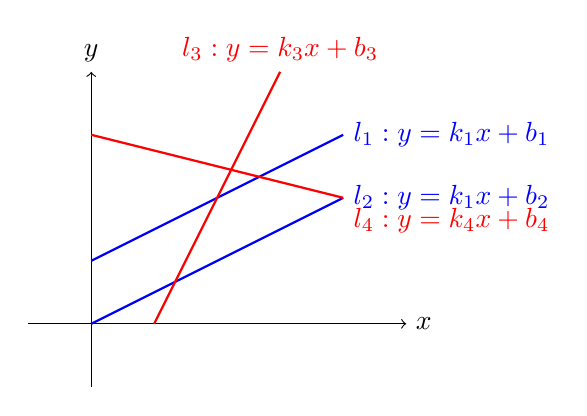
\begin{tikzpicture}[scale=0.8]
            \draw[->] (-1,0) -- (5,0) node[right] {$x$};
            \draw[->] (0,-1) -- (0,4) node[above] {$y$};

            \draw[thick, blue] (0,1) -- (4,3) node[right] {$l_1: y = k_1x + b_1$};
            \draw[thick, blue] (0,0) -- (4,2) node[right] {$l_2: y = k_1x + b_2$};

            \draw[thick, red] (1,0) -- (3,4) node[above] {$l_3: y = k_3x + b_3$};
            \draw[thick, red] (0,3) -- (4,2) node[below right] {$l_4: y = k_4x + b_4$};
        \end{tikzpicture}
    \end{minipage}
\end{theorem}

\begin{example}
    已知直线 $l: 3x + 4y - 12 = 0$ 和点 $A(1,2)$，求过点 $A$ 且与 $l$ 平行的直线方程，以及过点 $A$ 且与 $l$ 垂直的直线方程。
\end{example}

\v{8em}
